\section{Data pipeline} \label{sec:data}

To train an interactive world model that remains responsive to time-varying instructions and control signals, we construct a unified data engine that transforms heterogeneous raw videos into temporally localized training dataset. The engine consists of three stages: \textbf{data acquisition}, \textbf{data profiling}, and \textbf{multi-granularity annotation}. 
In the first stage, videos from different sources are normalized into a shared metadata schema. In the second stage, low-quality or semantically unsuitable samples are removed through technical filtering and VLM-based profiling. 
In the final stage, retained videos are converted into structured annotations, video-level global captions, and chunk-wise local captions. The design goal is to provide both global semantic context and local supervision for state updates. Each chunk combines reliable visual evidence with concise local-state descriptions, helping the model capture scene dynamics, interaction outcomes, and control-sensitive transitions.

\subsection{Data Acquisition}

Our corpus is assembled from three complementary sources: self-collected egocentric videos, synthetic data from games and Unreal Engine environments, and large-scale web videos~\cite{yang2026aoe,wang2025spatialvid,grauman2022ego4d,buildaiegocentric10k2025,damen2020epic,egodex,bansal2022my,jang2019epic}. Egocentric videos capture real-world first-person interactions and natural hand-object behaviors. Synthetic data provides accurate scene geometry and temporally aligned interaction signals, such as jumping, attacking, driving and flying. These signals are difficult to recover reliably from in-the-wild videos, but are important for learning controllable state transitions. Web videos provide scalable open-domain coverage and expose the model to long-tail visual distributions.

Before profiling, each raw video is converted into a standardized record containing source information and basic attributes for downstream processing. This mixed-source data curation strategy follows recent video world model data pipelines, which combine web-scale, synthetic, and action-conditioned data to improve both visual diversity and controllability~\cite{xiong2026actworld,lingbot-world,cosmos}.

\subsection{Data Profiling}

Raw videos differ in quality, viewpoint, and semantic content, so we first validate decoding, remove invalid samples, and detect shot boundaries. For long videos, we use TransNet V2~\cite{soucek2024transnet} to split them into temporally coherent clips, which are then filtered by basic constraints such as duration, resolution, and decoding stability.
After segmentation, we apply technical scoring filters as an inexpensive screening step. The score aggregates signals such as visual quality, luminance range, OCR-based text occupancy, motion statistics, and encoding stability~\cite{schuhmann2022aesthetic,wu2023exploring,cui2025paddleocr}. This stage is designed to remove clearly unsuitable clips while preserving enough high-quality candidates for later semantic filtering.

We then use a vision-language model to profile the retained candidate clips~\cite{qwen3.5,qwen3.6-35b-a3b,qwen3.6-27b}. VLM profiling produces two groups of attributes. The first group describes sample quality, including editing artifacts, and ambiguous visual evidence. The second group describes semantic content, including viewpoint, activity category, and interaction pattern. Technical filtering and VLM profiling serve different purposes, the former provides low-cost quality control, while the latter organizes the retained clips for data balancing and prompt routing.


\begin{figure}[t]
    \centering
    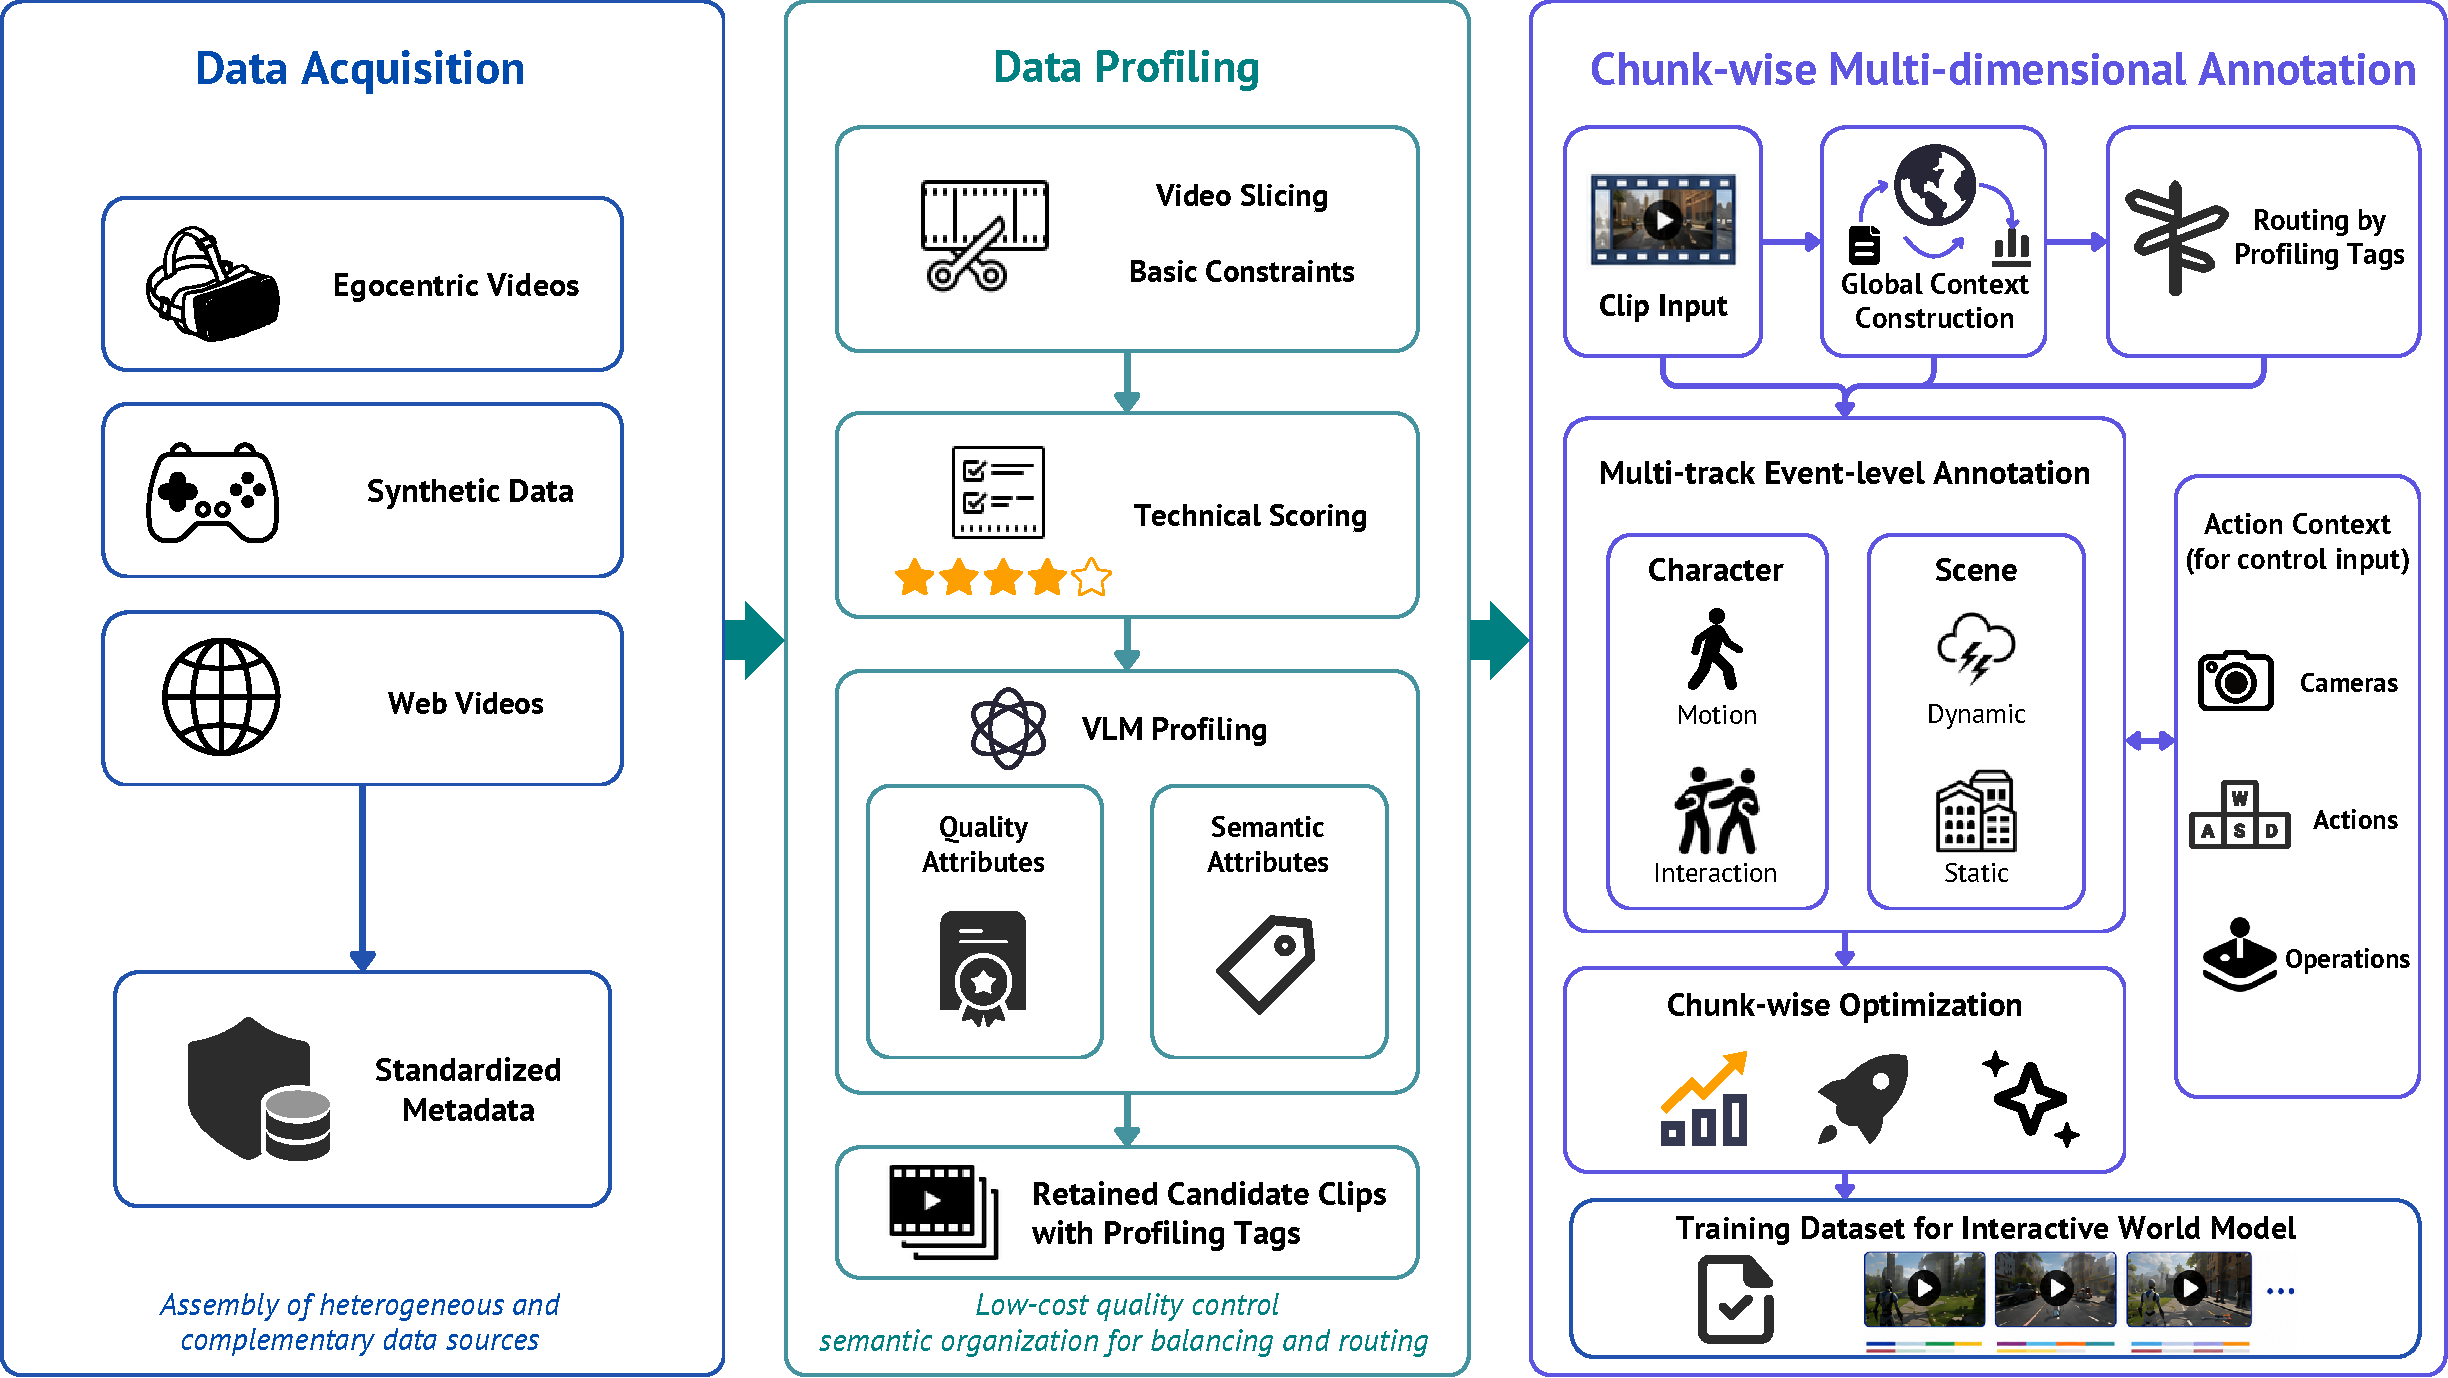
\includegraphics[width=\linewidth]{figures/data_engine.pdf}
    \caption{
    Overview of the proposed data engine. Heterogeneous raw videos are temporally segmented, filtered, and routed to category-specific annotation pipelines, producing optimized chunk-wise captions.
    }
    \label{fig:data_engine}
\end{figure}

\subsection{Multi-dimensional Video Annotation}

Existing video datasets often associate each video with a single global caption, which provides a video-level semantic summary of the scene, task context, and overall interaction trajectory~\cite{chen2026memdreamerdecouplingperceptionreasoning, zhang2026muss, wang2025koala, chen2024panda, tan2024vidgen, nan2025openvid, Yang2025ViMix14MAC}.
%
However, our model is designed for real-time interaction, where the conditioning signal may vary over time in response to user instructions or actions. 
Training only with global captions would therefore create a train--inference mismatch: the model would be required to follow localized instructions at inference time without having been exposed to comparable temporal conditioning during training.

To address this issue, we construct multi-dimensional annotations that combine video-level global context with temporally localized chunk-wise descriptions. 
Given a preprocessed video clip, our pipeline first establishes a stable global context, then produces event-level annotations for each temporal chunk, and finally composes these annotations into visually grounded and temporally aligned captions. This hierarchical design is consistent with recent interactive and causal video world models that leverage hierarchical captions or per-chunk semantic descriptions~\cite{meng2026causalcine,longlive_2.0,Yesiltepe_2026_CVPR}.

\paragraph{Multi-track event-level annotation} 
For each chunk, the annotation process is adapted according to the clip profile and available input modalities.
Rather than enforcing a single temporal boundary for all semantic attributes, we annotate multiple event tracks independently. These tracks cover subject visibility, motion state, interaction state, environmental dynamics, and static scene state. 
This decoupled representation reduces temporal ambiguity by preventing unrelated visual, interaction, and scene changes from being merged into a single description. 
When control signals are available, we use temporally aligned and semantically normalized action context as auxiliary evidence for chunk annotation. 
The action context mainly provides boundary cues and helps recover short interactions that may be missed by sparse visual sampling, while the final captions remain constrained by visible evidence to avoid speculative actions or state changes.

\paragraph{Chunk-wise optimization}
After event-level annotation, we compose active track states into chunk-wise captions and apply a lightweight refinement stage to improve terminology consistency and temporal smoothness. 
We further remove future-revealing, speculative, or redundant expressions, yielding visually grounded and temporally aligned chunk-wise annotations for training.